\title{Engineering Physics 253 Proposal - Das Pan}
\author{
        Alex Swift-Scott 30070122\\
                Andrew Dworschak 22620141\\
                Justin Kang 14819149\\
                Rahat Dande 17228140\          
}
\date{\today}

\documentclass[12pt]{article}
\usepackage{enumitem}
\usepackage[utf8]{inputenc}
\usepackage[english]{babel}
\usepackage[letterpaper, margin=1in]{geometry}
\usepackage{titling}
\usepackage{array}
\usepackage{longtable}
\usepackage{graphicx}
\usepackage{array}
\graphicspath{ {img/} }
\usepackage{csvsimple}
\newcolumntype{L}[1]{>{\raggedright\let\newline\\\arraybackslash\hspace{0pt}}m{#1}}
\newcolumntype{C}[1]{>{\centering\let\newline\\\arraybackslash\hspace{0pt}}m{#1}}
\newcolumntype{R}[1]{>{\raggedleft\let\newline\\\arraybackslash\hspace{0pt}}m{#1}}

\begin{filecontents*}{arm.csv}
Name,Purpose,Machining,Assembly
Supporting Beam,Bear the weight of the arm and anchor it stably to the base,A square beam of material ( or an I-beam) where holes are drilled through.,Will be anchored to the ground using 4 square brackets and hold up the arm using 2 connectors
Connector,To provide bearings and pivots for each of the arm’s parts,Laser cutting,Attached to the supporting beam by 3 screws
Big Gears,Gears that control each rod of the arm to achieve the desired motion,"Laser cutting with threaded holes, possibly to have screws held in place by epoxy once the design is finalized.",Screws/bolts will hold the gear in place while allowing it to rotate freely. The screws will not protrude from the outer edge of the gear
Small Gear,A gear to be driven by the motor that will not exceed its torque and also make sure the system rotates in the desired direction.,"Laser cutting with threaded holes, possibly to have screws held in place by epoxy once the design is finalized.",Screws/bolts will hold the gear in place while allowing it to be driven by a motor.
Top Rod,A rod used to provide the up and down motion in the sweep as controlled by a big gear,Laser cutting,To be fixed to a pivot joint on the connector and have a screw that is free to slide along the slot in the rod
Bottom Rod,A rod used to provide the out and in motion in the sweep as controlled by a big gear,Laser cutting,To be fixed to a pivot joint on the lower big gear.
Sweeper,Both rods will be attached by pivot joints to the sweeper. It will trace out a circular sweeping motion,"Laser cutting, broom made from fingers of a rubbery material yet to be determined.",To be attached to the top and bottom rods by a pivot joint.
\end{filecontents*} 

\begin{filecontents*}{Dustpan.csv}
Name,Purpose,Machining,Assembly
Pan,To carry and hold passengers from the pickup zone to the drop-off. Designed in a way that passengers can be swept into it like a dust pan.,A piece of sheet-metal to be cut on the waterjet cutter and then bent into shape using hand tools and machines.,Will be attached to the base of the robot by a pan-connector.
Pan connector,To attach the pan to the base of the robot in a way that the pan always stays as flat and close to the ground as possible.,A rubbery material yet to be determined that is cut into a narrow strip.,Glued to the edges of the pan and base of the robot.
Pushoff,A strip of material used to push the passengers off the dust pan and into the drop-off zone.,Waterjet cutting/laser cutting,Held to the back of the pan by an elastic band and winched forward by 2 pieces of string around either end.
Pulleys,"To  pull the pushoff in the correct direction, effectively ejecting passengers from the robot","A premade part, probably mechano",Attached to the pan at its corners.
Winch,A rod spun by a motor to  pull the pushoff in the correct direction,2 laser cut pieces with a hole in them and a rod cut to size,Fastened to the base of the robot and spun by a motor at the back end.
Base,The base of the robot where all of the circuitry and components are housed.,"A waterjet cut piece of metal that is bent using hand tools and machines, reinforced by several cross-bars along the underside.","A solid base where many different parts are fastened using bolts, glue and spot welding."
\end{filecontents*} 

\begin{document}
\begin{titlingpage}
\maketitle 
\begin{abstract}
\end{abstract}
\end{titlingpage}

\tableofcontents
\section{Executive Summary}
\subsection{The Problem}
The state of today’s roads is dire. The failure of the UBER automated vehicle
program has left passengers stranded, abandoned and worse, run over.
\subsection{Our Solution}
Our objective is to solve this problem, by efficiently picking up all stranded
passengers. The “Das Pan” will feature a sweeping arm that pushes
passengers into our “pans”, a holding area, where they will stay for the
duration of their ride.
\subsubsection{Design Specifications}
The Das Pan, at a weight $\approx$ 8lb consists of three main modules. 

\paragraph{Arms}The arms, supported by a beam of height ?, have a length of ?,
and sweep in a unidirectional fashion in such a way that they are able to push
the passenger into the pans, whcih have dimensions ? x ?.

\paragraph{Body} The body, which consists of a base for the arms, wheel wells
for the ? diameter wheels and a housing for the circuits, is the central
portion of our design. On both the left and right side of the body, we have two
large ? x ? pans for holding passengers.

\paragraph{Electronics}The electronics, which consists of a series of sensors, actuators, and a central microprocessor.  

\subsubsection{Target Performance}
Our final Prototype will be able to navigate the roads in an intelligent
Fashion, seeking out passengers by using the information it has at hand. In our
final mechanism, Das Pan should be able to complete a passenger retrieval action
in less than 10 seconds. 

\section{Preface}
\par Work for this proposal was divided among our team using an excel
spreadsheet. We began outlining the subsections of our report, using the outline
provided in lectures. Subsections were defined from all pertinent information.\\

Once we defined subsections, as a team, we determined which member would be
most knowledgeable about specific subject, and assigned them to the task.\\

All sections began by creating a set of figures and tables. We shared these
tables and figures with one another, and provided feedback, continually making
modifications until all members were satisfied with the result.\\

Throughout this process, we sought out the help of our mentors and instructors,
namely Pam <insert last name here>, Jon Nakane, and Bernhard Zender, who guided
us in the formatting and the technical writing of this document. 

\section{Overview of Basic Strategy}
\par Our objective is to create a simple yet effective robot. We believe that a
plain and straightforward design is a successful design.
\subsection{Mechanical Overview}
\par Precision plays a vital role in traditional passenger retrieval. We sought
to engineering out precision.  We came up with a broom and dust-pan design.  Our
arm will sweep passengers off their podium and drag them into our dust-pans. 
This does not require the precision of other candidate mechanism such as
forklifts, since the broom can span a wide range. This also avoids destroying
houses since the bristles of the broom will be elastic and will deform around
rigid structures. 
\subsection{Electrical Overview}
\par We plan on modularizing our electrical circuits such that each circuit that
performs an atomic function (ex. H-Bridge, IR detect) is on its own board.  We
think that an encapsulated and modularized circuit design will allow us to
individually test components.  Such components are also easily replaceable.
\subsection{Software Overview}
\par We will store a graph representation of the playing surface in memory for
decision making during navigation. Each node signifies an intersection on the
surface, and each edge represents a path. We will use dynamic weights to decide
which path to take.  The weights depend on the likelihood of a passenger being
in an edge, the presence of a passenger at an edge, and the path to the drop off
area.  We will adjust weights as we pick up a passenger so the weight of the
edge from which we picked up the passenger is decreased, and the weights of the
edges toward the drop off are increased.  This means that once we are at
capacity, the weights will make it more favourable for the robot to navigate to
the drop off area rather than pick up another passenger.\\

Storing the surface in memory allows for smarter decision making and will reduce
our dependency on detecting IR signals to find the drop off area.
\section{Chassis}
\begin{figure}[h]
\centering
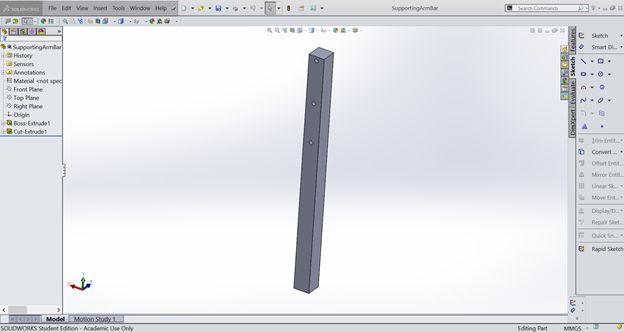
\includegraphics[scale=0.5]{arm.png}
\caption{Model of the robot in its entirety}
\label{fig:4.1}
\end{figure}
\begin{itemize} 
  \item The TINAH and other electrical components will be housed at the back of
  the robot for easy access. 
  \item Before the final assembly, parts will be held together by screws to
  facilitate disassembly.
  \item The estimated mass of the robot is 8 lbs broken down as follows:
  \begin{itemize} 
    \item Arm: 2 lbs
    \item Dust pans and dragging parts: <1 lb
    \item Main body and circuitry: 5 lbs
  \end{itemize}
\end{itemize}
\subsection{Components}
Refer to Appendix A for images of all parts
\subsubsection{Arm}
\begin{longtable}{|L{2cm}|L{4cm}|L{3cm}|L{3cm}|}
\hline
    \bfseries Name & \bfseries Purpose & \bfseries Machining &\bfseries Assembly
    % specify table head
    \csvreader[head to column names]{arm.csv}{}% use head of csv as column names
    {\\\hline  \Name & \Purpose & \Machining & \Assembly }
    \hline
\end{longtable}
\subsubsection{Dust Pan}
\begin{longtable}{|L{2cm}|L{4cm}|L{3cm}|L{3cm}|}
\hline
    \bfseries Name& \bfseries Purpose & \bfseries Machining &\bfseries Assembly
    % specify table head
    \csvreader[head to column names]{Dustpan.csv}{}% use head of csv as column
    % names
    {\\\hline  \Name & \Purpose & \Machining & \Assembly }
    \hline
\end{longtable}

\subsection{Redesign Potential and Flexibility}
Where is this?
\subsection{Estimated Final Specifications}
Where is this also?
\section{Drive and Actuator System}
\par There are 8 actuators total in our design: a pair of geared Coleman motors to power the wheels (bidirectional), a pair of geared Coleman motors to move the arms (unidirectional), a pair of un-geared Coleman motors to power the pusher winches (bidirectional) and a pair of servo motors to lock the pushers in place. \\
\subsection{Drive Mechanism and Transmission}
\par There are two powered wheels, which are controlled independently to allow for tape following, turning and driving in reverse. In addition, there is an unpowered ball-and-socket roller to provide a third point of contact. To maximize control in tape following, the wheels were placed on the very back end of the chassis. To maximize torque while turning, the wheels were placed with the largest possible distance between them (12''). The roller was placed at the very front of the robot, along the centerline, to maximize its distance from the driving wheels and improve stability. \\ \par 
The placement of the wheels, drive motors and transmission is illustrated below: \\
//TODO: INSERT DIAGRAM + CALULATION \\
\par Therefore, in order to accelerate the robot at a maximum acceleration of ${0.5 \frac{m}{s^2}}$, the drive motors must exert a torque of \_\_\_. This will consume \_\_\_ W of power. To maintain constant velocity, the motors must exert a torque of \_\_\_. This will consume \_\_\_ W of power. \\
\subsection{Steering}
\par The robot's pair or arms and passenger-collection pans
allows it pickup and drop off passengers to either side without turning away
from the tape line in the path's center. In addition, the robot will be able to drive in reverse, allowing it to enter and exit dead-end streets without needing to turn. Because of this, the robot will never need to turn under any circumstances other than at intersections in the path. \\ \par Therefore, in order to make a turn, the robot must be able to detect an intersection, right itself onto the correct tape line once the turn is complete, and be mechanically capable of turning itself. To detect the intersection, the robot will read the output of branch-detection QRDs placed near the front right and front left corners of the chassis. To right itself, it will rely on the normal tape-following QRDs. \\ \par The turning mechanism is illustrated below: \\
//TODO: INSERT DIAGRAM + CALCULATIONS \\
\par Therefore, in order to begin turning and maintain a constant angular speed,  the motors must exert a torque of \_\_\_. This will consume \_\_\_ W of power. \\ \par 
Considering this and the previous constraints on torque calculated for driving and accelerating, the gear ratio should be approximately \_\_\_. \\
\subsection{Arm Mechanism}
\par The left and right sides of the robot both have an identical arm, so that passengers can be retrieved from either direction without changing the yaw of the arm. The arm is jointed and ends in a brush (made of rubber tines or fibres strong enough to push a passenger but flexible enough to give way when brought against a building or curb). The joint of the arm are designed so that, with a single rotation of the large, arm-supporting gears, the brush will trace out a horizontal path (allowing it to “sweep� passengers into the pans). \\ \par 
\par This mechanism is illustrated below: \\
//TODO: INSERT DIAGRAM + CALCULATIONS \\
\par Therefore, in order to move the arm through 1 complete cycle in 5 seconds (unobstructed by objects in path of brush), the motor must exert a maximum torque of \_\_\_.
\subsection{Pan Mechanism}
\par The left and right sides of the robot both have identical pans, which consist of a lightweight surface of sheet metal attached to the chassis by a narrow rubber strip. The pan also has a winch-powered pusher and pulley mechanism to expel passengers at the drop-off zone by pushing them out of the pans. In addition, if the pusher strip is held in place by a locking servo, the winches will instead pull the pans up slightly, pulling them off the ground to reduce friction and ensure that passengers don't fall out during transport. \\ \par 
This mechanism is illustrated below: (the pans are simple and required few calculation beyond basic size) \\
//TODO: INSERT DIAGRAM + CALCULATIONS \\

\subsection{Motor Table}
(All required values are estimated for 1 round of competition) \\ \\
\hspace*{-5pt}\makebox[\linewidth][c]{
\begin{tabular}{| L{8em} | L{8em} | L{6em} | L{8em} | L{4em} |}
\hline
Motor type & Function & Required voltage & Required power & Required current \\
\hline
Geared Barber Coleman motor (FYQF 63310-9) x2
Drive individual wheel both forward and reverse & ~12V & (supplied by LIPO) & Driving: \newline Accelerating: \newline Turning: \newline Stationary: ~ 0 W\newline \newline Time spent in each state: D:A:T:S = 4:2:3:5, & TODO \\
\hline
Geared Barber Coleman motor (FYQF 63310-9)
x2 & Drive individual arm through its path cycle, forward only & ~12V (supplied by LIPO)
 & 1 cycle: \newline
Approx. 20 cycles performed during 1 round & TODO \\
\hline
Un-geared Barber Coleman motor (FYQM 63100-51)
x2 & Turn winch to extend individual pusher (or lift pan, if pusher is locked) & ~12V (supplied by LIPO) & Lower pan:   (approx. 10x / round) \newline Raise pan:    (approx. 10x / round) \newline Expel passengers:  (approx. 4x / round) \newline & TODO \\
\hline
TowerPro 9g micro servo (SG90) & Lock pusher in place so that it can't be extended & ~5V (supplied by TINAH) & Lock/unlock:   (approx. 10x / round) & TODO \\
\hline
\end{tabular}
}

\section{Electrical Design}
\subsection{TINAH I/O Allocation}
\begin{longtable}{| L{7em} | L{3em} | L{25em} |}
\hline
Type & Name & Use (Connected to) \\
\hline
Analog input & A0 & Front left passenger-locating IR sensor PCB signal \\
\hline
Analog input & A1 & Back left passenger locating IR sensor PCB signal \\
\hline
Analog input & A2 & Front right passenger locating IR sensor signal \\
\hline
Analog input & A3 & Back right passenger locating IR sensor signal \\
\hline
Analog input & A4 & Left arm feedback potentiometer signal \\
\hline
Analog input & A5 & Right arm feedback potentiometer signal \\
\hline
Analog input & A6 & Unassigned (defaults to knob 6) \\
\hline
Analog input & A7 & Bumper contact detection PCB signal (if unused, defaults to knob 7) \\
\hline
Digital output & 0 & Input of Left arm motor control PCB \\
\hline
Digital output & 1 & Input of Right arm motor control PCB \\
\hline
Digital output & 2 & Unassigned (defaults to Serial 1 - RX) \\
\hline
Digital output & 3 & Unassigned (defaults to Serial 1 - TX) \\
\hline
Digital output & 4 & Left front bumper contact switch \\
\hline
Digital output & 5 & Right front bumper contact switch \\
\hline
Digital output & 6 & Left rear bumper contact switch \\
\hline
Digital output & 7 & Right rear bumper contact switch \\
\hline
Digital output & 8 & Left arm brush contact switch (possibly redundant) \\
\hline
Digital output & 9 & Right arm brush contact switch (possibly redundant) \\
\hline
Digital output & 10 & Unassigned \\
\hline
Digital output & 11 & Left driving QRD PCB signal \\
\hline
Digital output & 12 & Right driving QRD PCB signal \\
\hline
Digital output & 13 & Rear rotation QRD PCB signal (possibly redundant) \\
\hline
Digital output & 14 & Left branch detection QRD PCB signal \\
\hline
Digital output & 15 & Right branch detection QRD PCB signal \\
\hline
Motor enable & PWM0 & Unassigned \\
\hline
Motor enable & PWM1 & Unassigned \\
\hline
Servo output & PWM2 & Unassigned \\
\hline
Servo output & PWM3 & Unassigned (also controls buzzer) \\
\hline
Motor enable & PWM4 & Unassigned \\
\hline
Motor enable & PWM5 & Unassigned \\
\hline
Direct motor outputs and indicators & Motor 0 to Motor 3 & Unassigned (Barber Coleman motors used required more voltage than the 9V maximum the TINAH can provide) \\
\hline
Motor control output & Motor 0 & Motor DIR, Motor !DIR, and Motor Enable pins to input of Left drive motor H-bridge PCB inputs \\
\hline
Motor control output & Motor 1 & Motor DIR, Motor !DIR, and Motor Enable pins to input or Right drive motor H-bridge PCB inputs \\
\hline
Motor control output & Motor 2 & Motor DIR, Motor !DIR, and Motor Enable pins to input of Left pan winch control PCB inputs \\
\hline
Motor control output & Motor 3 & Motor DIR, Motor !DIR, and Motor Enable pins to input of Right pan winch control PCB inputs \\
\hline
Servo motor output & Servo 0 & Signal to left pan locking servo \\
\hline
Servo motor output & Servo 1 & Signal to right pan locking servo \\
\hline
Servo motor output & Servo 2 & Unassigned \\
\hline
\end{longtable}
\subsection{Electrical Design}
All PCBs will be soldered onto perforated board by the same convention: all
components flat, and all wires straight and colour-coded to indicate function\\

\begin{longtable}{| L{7em} | L{7em} | L{7em} | L{7em}|}
\hline
PCB name and number & Function & Material and Size & Connections\\
\hline
Passenger-locating IR sensor PCB \newline X4 identical copies: \newline Front
left \newline Back left  \newline Front right  \newline Back right & Read directional IR levels at sensor, filter out noise and DC components of signal, amplify 1 kHz component of signal, convert to DC.
Output: DC analog signal proportional to sensor distance from IR emitter & - standard PCB backing
\newline - front copy and back will be wired onto the same 3’’ x 2’’ board
(making for 2 boards total) & For each board (x2): \newline GND (MTA-100
connector) \newline +5V (MTA-100) \newline +15V (MTA-100) \newline -15V
(MTA-100) \newline IR sensor signal \newline  (x2) (from IR sensor)
\newline Output signal (x2)(MTA-100)\\
\hline


\end{longtable}
\subsection{Physical Wiring Table}

\section{Strategy, Algorithms and Software}
\subsection{Tape Following and Navigation}
\subsubsection{Machine State}
There are two main states that our robot will inhabit for most of the duration
of the competition - roam search empty, and roam search full - with the main
difference between the two being the absence and presence of a passenger
respectively.\\

When in roam search empty, which is the starting state of the robot, the robot
will wander the playing field in search of a passenger using pre assigned
weights for each path.  Once a passenger is detected, the robot will attempt to
pick up the passenger.  If the attempt is successful the robot will go to roam
search full state.\\

Every time a passenger is picked up, the weight of the path from which the
passenger was picked will be reduced and weights leading to the drop off area
will be increased.  In roam search full, the robot will still be able to detect
passengers and pick them up.\\

Eventually, with enough passengers, it will be more favourable for the robot to
go to the drop off area.  The weights of the path will reflect this since the
weights of the paths on the playing fields are adjusted each time a passenger is
picked.  Since our robot will have passengers on both sides, it is possible that
the robot is still full after the drop off operation.  At this state, the robot
will return to roam search full.  If the robot is empty it will return to roam
search empty.\\

In the last 30 seconds of the competition, if the robot is in roam search full
state, weights will also be adjusted to favour the drop off area.  While in roam
search empty the weights of the paths reflect the probability of a passenger, in
roam search full they also represent the urgency of a drop off - whether due to
capacity or due to time.\\

At any time, if the robot senses that a collision is eminent, it will stop its
operation and attempt to navigate away from the collision.\\

Please refer to the state diagram below for a summary.

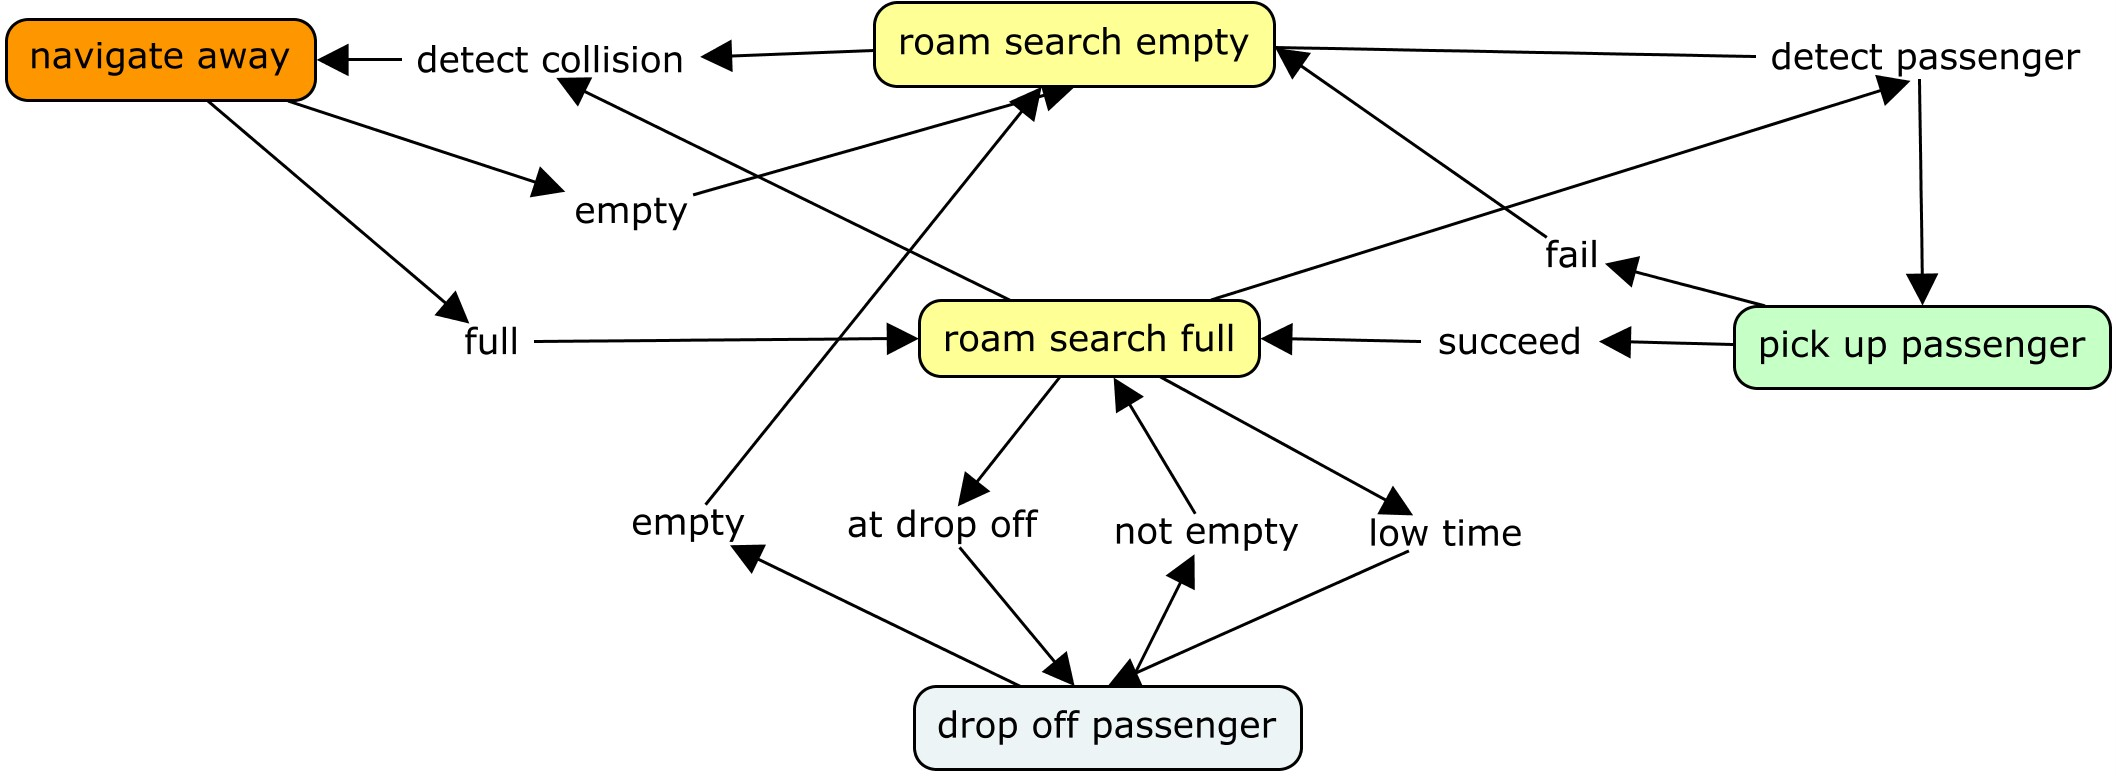
\includegraphics[scale=0.2]{robot-state-diagram}
We will use PID control to follow the tape on the playing surface.  We will
finely tune the proportional, integral, and differential error gains with much
data and experimentation.

\subsubsection{Graph Based Navigation}
We plan on storing a discrete graph representation of the playing surface in
memory on the TINAH.  Each intersection on the playing surface will be a node,
and each path between the intersections will be an edge.  The graph will be
weighted, but not directional.  The weights of the graph will characterize the
likelihood of a passenger being on a certain edge.\\
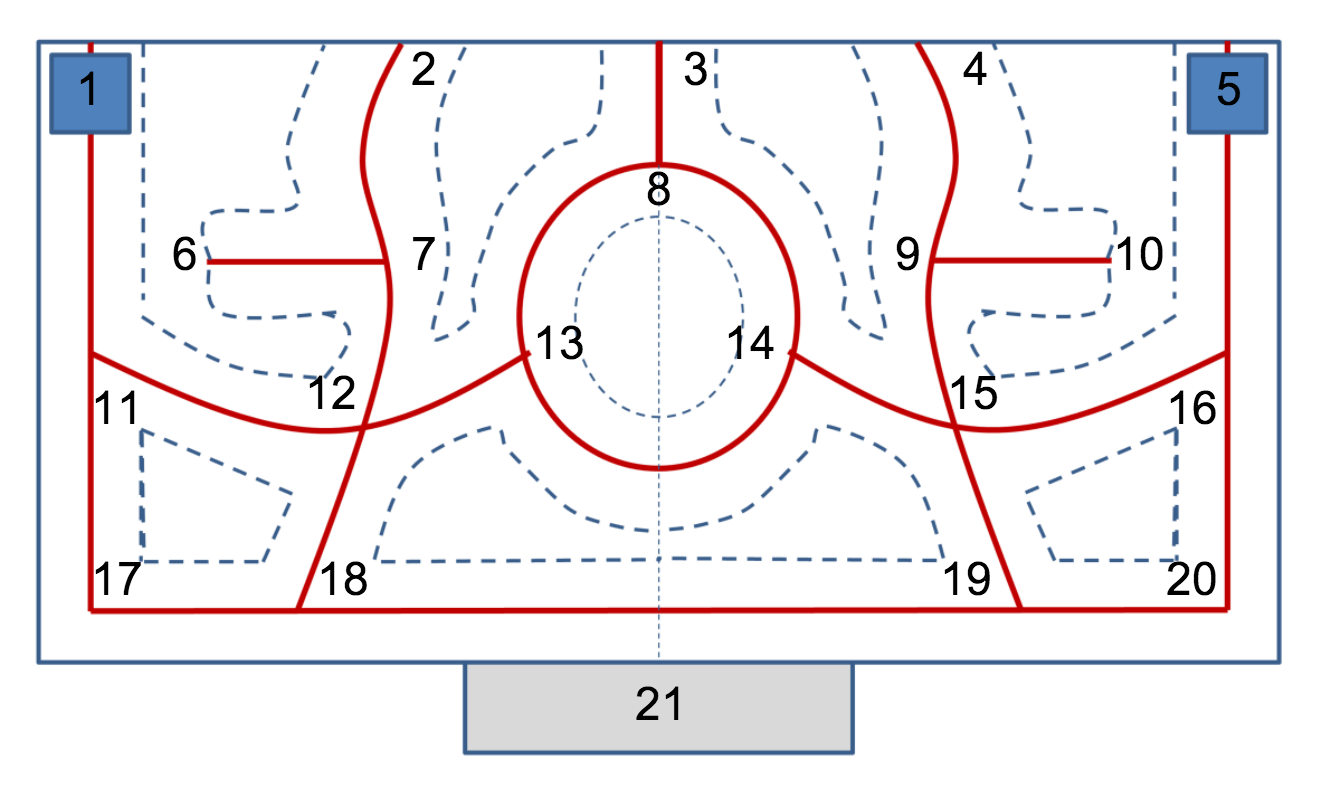
\includegraphics[scale = 0.5]{map}
\newline
The weights of the graph will also be dynamic, changing based on the state of
the robot.  The initial weights will be based on the number of possible
locations for a passenger.  Once we pick up a passenger from a certain edge, the
weight for the edge will decrease.  If we the robot has a passenger, the weights
for the edges in the shortest path to the destination will be increased.  The
weights will also be ignored if the robot senses a passenger’s beacon at some
edge.\\
\begin{center}
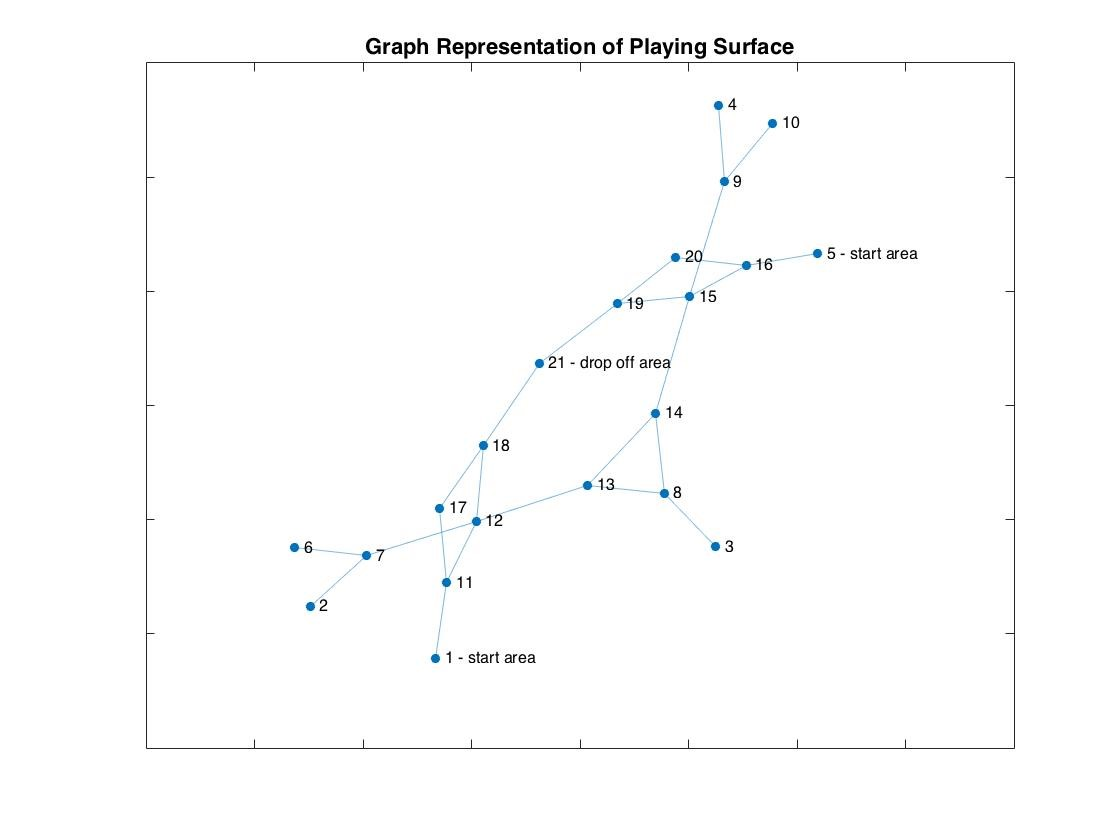
\includegraphics[scale = 0.4]{graph}
\newline
\end{center}
By storing the playing surface in memory, we hope to reduce the robot’s
dependency on IR signals for self-location and navigation.  Storing the playing
surface is also advantageous in making decisions based on history and location.
\subsection{Passenger Detection}
The robot will use IR signals to detect passengers.  As mentioned before, if a
passenger is detected at any time, the weights of the graph will be ignored and
the robot will attempt to pick up the passenger.
\subsection{Collision Detection}
If the robot detects a collision, it will escape whatever state it is in and
attempt to navigate away from the collision.

\section{Risk Assessment and Contingency Planning}
\subsection{Risk Assessment}

\begin{longtable}{| L{7em} | L{7em} | L{7em} | L{7em} | L{6em} |}
\hline 
Risk Condition & Probability of Occurrence & Impact to Project & Change to Work Plan & Expected Date of Risk Decision \\
\hline
Robot get’s lost in map due to failure to detect the presence of an intersection
& (Based on Jon’s expertise) Unlikely to occur so long as speed is kept within a
reasonable range & Robot will be unable to return passengers to base during the
competition & Create a structure that reaches the height of the destination
beacon and & Week two of robot construction \\
\hline
During the competition a passenger falls out of its containment area during
turning or otherwise& Dependant on the rigidity and geometry of container &
Robot will loose the current passenger, but will be able to continue thereafter.
& Minor Problem - increase side wall length

Major Problem \newline - further increase the walls of the containment area
while redesigning the arm to ensure the passengers can land in this modified
container & Week 2 of robot construction\\
\hline
During collision on competition day the extruding flaps in our design are more
likely to be damaged than the chassis. If the flaps are damaged during a
collision, the robot’s passenger containment mechanism could be compromised & It
is likely that during a collision, these low-hanging flaps will be impacted,
however, by using stronger materials, and ensuring the flaps have reliable
fixtures joining them to the main chassis we can mitigate this risk.& Minor
damage will likely cause little impact on the robot's functionality, except for
perhaps decreasing the integrity of the passenger containment area, and thus
increasing the risk of passenger loss &Increase the number of collision sensors
to prevent collisions in the first place & Final week of robot construction \\
\hline
Risk that the maximum reach of the arm will limit our capacity to pick up
passengers when they are far away & Depending on the geometry of the track and
placement of the passengers.& Inability to retrieve passengers located too far
from the midline of the track & Changing the arm’s length and range of motion.
This will be made easy due to the arm’s modular design & Decision will be made
once track has been finalized\\
\hline 
Risk of catching or stalling the arm on obstacles or buildings when operating&
Very unlikely because the arm only operates when the robot is stationary, and
the brush is designed to give way to obstacles.& Most likely temporary
disruption of the arm’s or robot’s motion, possibly moderate damage to the arm.
&Changes to the flexibility of the brush or design and range of motion to avoid
future catching & Decision can be made once design is finalized while testing
robot on track.\\
\hline
Risk that the arm’s sweep knocks the passenger away from the arm’s reach, fails
to push it all the way to the pan, or fails to push it over the pan’s edge &
Probably unlikely given the arm’s motion shouldn’t allow this. It is difficult
to say without testing&Failure to retrieve the passenger, possibly knocking it
into the path or off the arena& Change the structure of the brush and motion of
the arm. If necessary, add more degrees of freedom to the arm & During the
testing and development of the arm over the next few weeks\\
\hline
\end{longtable}

\subsection{Mitigation and Contingency Planning}
In order to prevent our robot from getting lost, due to it’s lack of a
destination beacon detector, we will ensure that we have a large safety factor
on our tape IR detection. We will engineer our navigation systems such that it
can perfectly detect intersections while traveling at top speed. This will
greatly mitigate the risk of getting lost due to a failure of the intersection
detection mechanism. \\

Furthermore, if time permits, a beacon detector may be implemented in order to
verify the state of our robot’s navigation system.\\

We can mitigate the risk of losing passengers by ensuring that  we use a
material with a high coefficient of static friction for the surface of our
passenger containment area. \\

By improving our collision detection systems we can reduce the risk of damage
due to collision. Furthermore, by protruding the anterior and posterior portions
of our robot, we can ensure that they take the brunt of most impacts.\\

To mitigate the risk of a limitation due to arm length, we will ensure that our
design will be as modular as possible
\section{Tasklist, Major Milestones, Team Responsibilities}
\subsection{Task List}
\subsubsection{Construction}
\begin{enumerate}
\item Construct chassis (without arms) and mount drive and transmission systems
\item Assemble all QRD mechanisms and affirm they function properly
\item Attach QRD and motor electrical mechanisms to chassis, achieve
tape-following
\item  Attach functional collision-detection bumpers to chassis
\item Assemble arm, confirm it retrieves passengers properly by itself
\item Assemble and attach pan mechanism to chassis, confirm it lowers/raises and
pushes properly 
\item Combine all elements into fully functional robot, affirm
that all components still work when operating simultaneously
\end{enumerate}
\subsubsection{Software Development}
\begin{enumerate}
\item Develop and optimize tape-following software for speed, stability and
  corner-following 
\item Develop an internal representation of the playing surface
\item Write the code to actuate the arm
\item Implement graph based navigation
\item Develop collision response software and confirm it functions in all
circumstances
\end{enumerate}
\subsubsection{Interfacing, Testing and Refinement}
\begin{enumerate}
  \item Successfully detect passenger at a distance, navigate to passenger and
  retrieve passenger consistently for a variety of passenger locations 
  \item Successfully navigate to destination area and drop off all passengers
  consistently 
  \item Successfully respond to collisions during every phase of operation
\item Optimize competition routine for number of passengers retrieved per unit
time
\end{enumerate}
\subsection{Miltestones}
\begin{enumerate}
  \item Each independent component is fully functional
 \item Having a fully functional ‘Das Pan’, containing all complete modules
\end{enumerate}
\subsection{Team Responsibility}
**gannt
\section{Document Contribution Summary}

\begin{longtable}{| L{8em} | L{5em} | L{5em} | L{5em} |}
\hline
Document Section & Draft Writers & Editors & Comments \\
\hline
Executive Summary& Justin &  Rahat & \\
\hline
Preface & Justin & Justin, Rahat & \\
\hline
Overview of Basic Strategy & Rahat & Justin & \\
\hline
Chassis & Andrew & Justin, Rahat & \\
\hline
Drive and Actuator Systems & Andrew, Alex & Justin & \\
\hline
Electrical Design & Alex & Justin & \\
\hline
Strategy Algorithms and Software & Rahat & Justin & \\
\hline
Risk Assesment and Contingency Planning & Justin & Rahat & \\
\hline
Tasklist & Justin & Alex , Rahat & \\
\hline
Appendix A & Andrew & Justin & \\
\hline
\end{longtable}

\appendix
\section{Solidworks Models of Parts} \label{App:AppendixA}
\subsection{Arm}
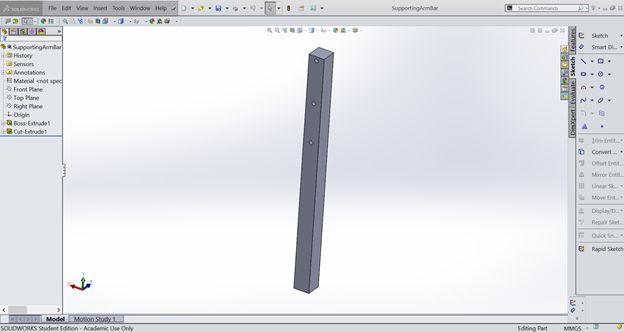
\includegraphics{arm}
\subsubsection{Connector}
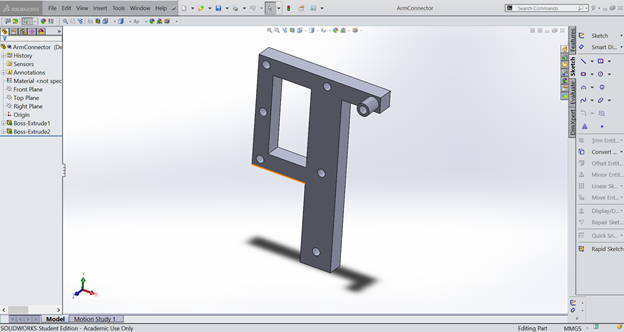
\includegraphics{connector}
\subsubsection{Big Gears}
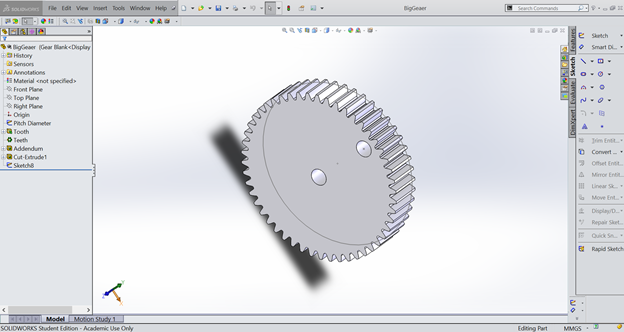
\includegraphics{gear}
\subsubsection{Small Gears} 
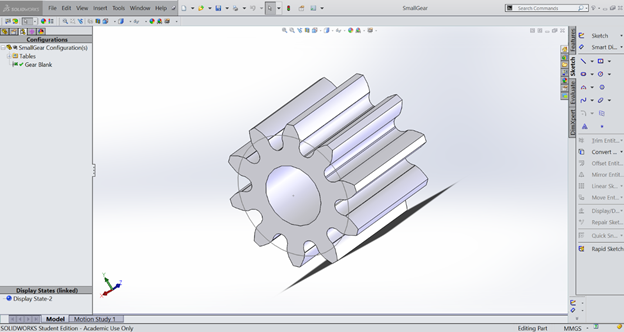
\includegraphics{gear-small}
\subsubsection{Top Rod}
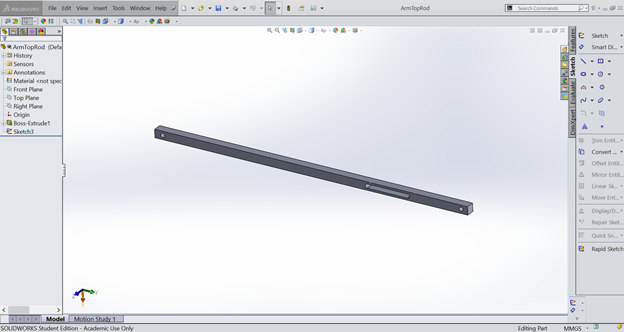
\includegraphics{top-rod}  
\subsubsection{Bottom Rod}
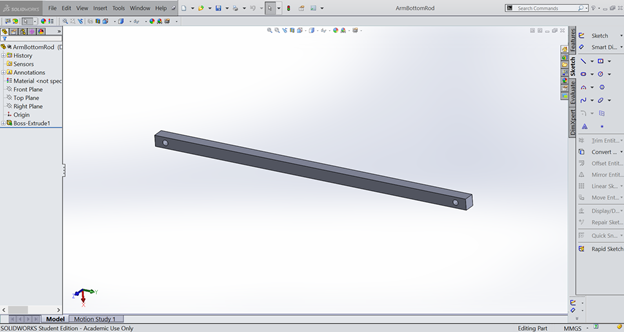
\includegraphics{bottom-rod}
\subsubsection{Sweeper}
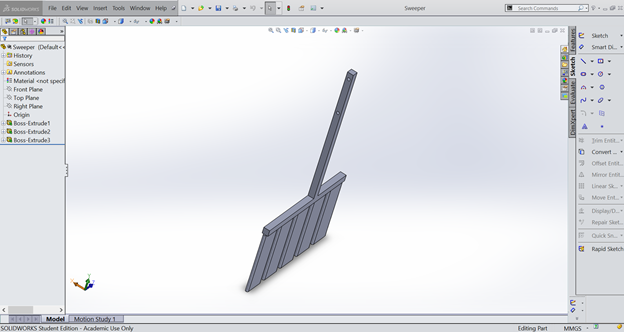
\includegraphics{sweeper}
\subsection{Dust Pan}
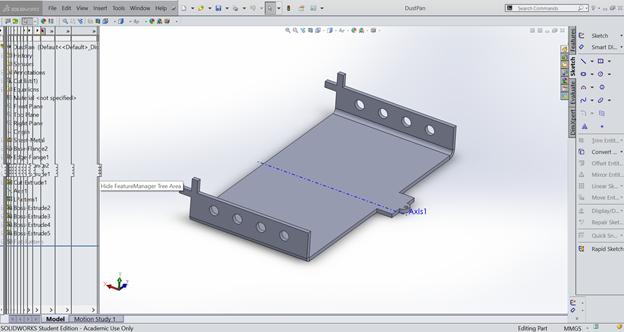
\includegraphics{dust-pan}
\subsubsection{Pan Connector}
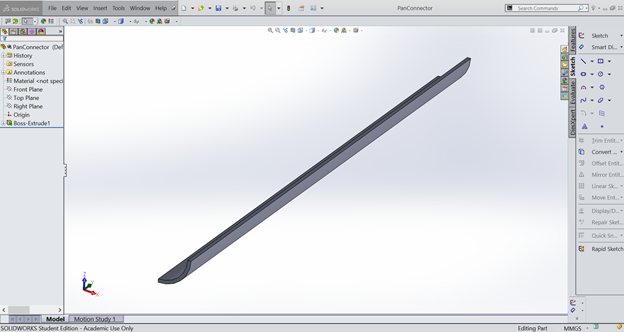
\includegraphics{pan-connector}
\subsubsection{Push-off}
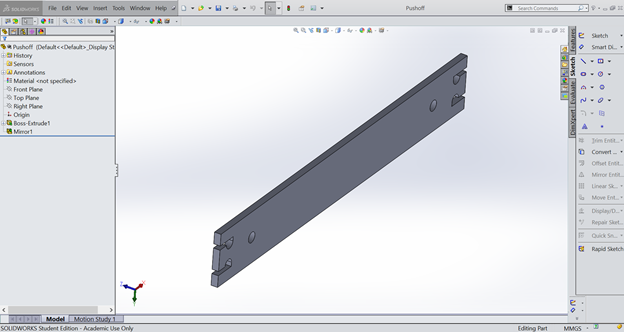
\includegraphics{pushoff}
\subsubsection{Pulleys}
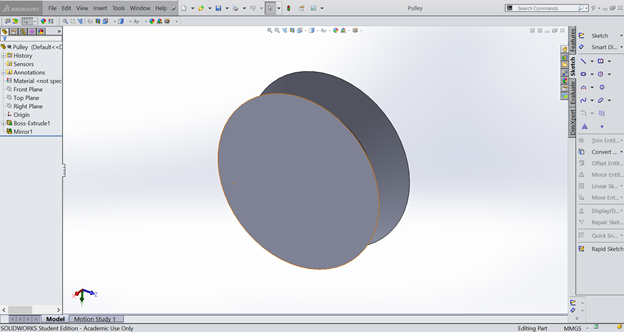
\includegraphics{pulleys}
\subsubsection{Winch}
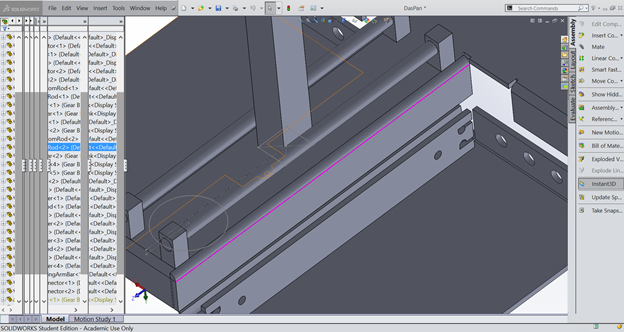
\includegraphics{winch}
\subsubsection{Base}
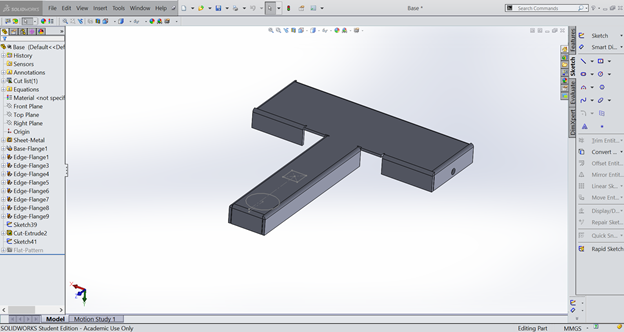
\includegraphics{base}
\end{document}